\chapter{Memória}
De uma maneira geral, quando um processo é criado, sua imagem (ou parte dela) é armazenada em memória, onde a as instruções e os dados que estão sendo manipulados em um determinado instante são carregados na CPU. Os dados alterados são escritos em memória continuamente e os mais permanentes são armazenados em disco.

Um programa fonte apresenta instruções contendo endereços simbólicos, definidos pelo programador. Após o processo de compilação e montagem, o programa agora apresenta endereços relocáveis, construído em relação ao início do módulo onde são definidos. Após a \textit{linkagem}, o programa agora possui os endereços absolutos, único para o programa como um todo. Finalmente, com o \textit{loader}, quando o programa é carregado para a memória, os endereços físicos são efetivamente definidos. % TODO: ver se essa última sentença tá certa

\section{Gerenciamento}
O gerenciamento de memória é implementado pelo \textbf{gerente de memória}, responsável por definir e implementar a política de gerenciamento de memória do SO. Além disso, independente desta política, o gerente deve controlar a alocação das porções de memória aos processos, liberando-as quando estas não forem mais necessárias. As técnicas de gerênciamento são três: \textit{monitor residente}, \textit{multiprogramação} e \textit{memória virtual}.






\subsection{Monitor Residente}
Em sistemas monoprogramados, a memória é geralmente dividida em duas áreas: uma para o usuário e outra para o sistema operacional.

Dessa forma, apenas um processo usuário está ativo por vez, pois a área de usuário é destinada a um processo apenas. Da mesma forma, a área do SO é ocupada por ele, o qual está sempre ativo.

Entretanto, é necessário um \textit{hardware} adicional, o qual vai impedir que processos de usuário invadão a área de memória do SO. É instaurada uma barreira, delimitando as áreas de memória, e a todo cálculo de endereço do processo usuário, o resultado é checado. A Figura \ref{fig:memory-fence} resume o processo.

\begin{figure}
  \centering
  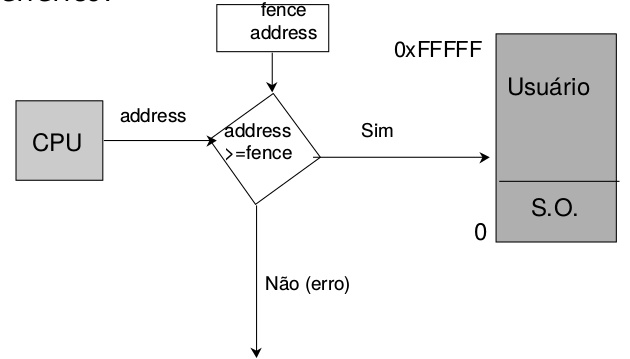
\includegraphics[width=0.65\textwidth]{memory-fence}
  \caption{O processo na CPU tentar acessar um endereço da memória. O \textit{hardware} checa se este endereço respeita o limite de área de memória do SO, liberando o acesso em caso positivo ou lançando um erro em caso negativo}
  \label{fig:memory-fence}
\end{figure}

Como \textbf{vantagens}, esta técnica tem implementação simples, pois só há um pequeno componente de proteção sendo usado. Além disso, os serviços do sistema operacional podem ser utilizados, como \textit{drivers}, interrupções, etc..

Como \textbf{desvantagem}, temos uma CPU sub-aproveitada, onde o sistema pode ser apenas mono-usuário e mono-tarefa






\subsection{Multiprogramação}
Multiprogramação é ofertada pela maioria dos computadores, onde vários processos coexistem na memória, havendo a necessidade da proteção de suas respectivas áreas de memória, evitando que um processo acesse a área de outro.

Logo, é lançado mão dos \textbf{registradores de base e limite}, definido dois limites de memória para o processo. Durante a execução, cada endereço usado para acessar a memória é adicionado ao valor contido no registrador de base, afim de obter o endereço físico onde o dado reside. Este registrador implementa a relocação.

Caso o endereço ultrapasse o valor do registrador limite, um erro é emitido. Assim, este registrador implementa a proteção de memória.







\subsection{Memória Virtual}
A memória virtual surgiu como uma solução para o problema de se alocar espaço em memória para um processo que não cabe inteiramente nela. Ou seja, temos um \textbf{processo com tamanho maior que o da memória física}.

A solução é quebrar o processo em unidades menores, carregando-as a medida que elas são necessárias. O problema é quem vai quebrar o processo: o programador ou o sistema operacional? Caso for o primeiro, temos um \textit{overlay} e do segundo, nasceu a memória virtual.

Proposto em 1961, é o método mais comum hoje em dia ao logo dos SO atuais, sendo um mecanismo genérico sendo suportado tanto por sistemas mono e multiprogramados. Logo, a idéia é referenciar mais endereços virtuais e não endereços físicos. Logo, parte do SO a responsabilidade de definir os módulos de memória e suas alocações.

\textbf{O número de endereços virtuais depende da capacidade de endereçamento da máquina} e do suporte do SO. Na execução de cada instrução, os endereços virtuais devem ser traduzidos para endereços físicos, o que exige um cálculo. Temos dois modelos para implementação da memória virtual:

\begin{itemize}
  \item \textbf{Paginação:} divide a memória física e a memória virtual em unidades de \textbf{tamanho fixo};

  \item \textbf{Segmentação:} divide a memória física e a memória virtual em unidades de \textbf{tamanho variável}.
\end{itemize}

Para ilustrar o possível espectro de endereços virtuais, supomos um arquitetura de 32 \textit{bits}. Logo, um processo pode endereçar até $2^{32} - 1$ endereços, independente da memória física.





\section{Espaço de Memória}

\subsection{Swapping}
\begin{definicao}{\textit{Swapping}}
  Movimento de processos \textbf{ativos} da memória para o disco e vice-e-versa.
\end{definicao}

Geralmente, a memória disponível no computador não é capaz de armazenar todos os processos ativos em um dado instante. Como não há espaço físico na memória, devemos colocar alguns processos ativos em disco. Normalmente, existe uma área em disco reservada para tal, chamada de \textbf{área de \textit{swap}}.

Definimos o movimento de memória para o disco como \textit{swap-out}. O movimento de disco para memória é o \textit{swap-in}.



\subsection{Alocação de Espaço}
O problema da alocação de espaço para processos é o problema de determinar a quantidade de memória que devemos reservar para um processo. Em sistemas onde um processo tem tamanho fixo, alocamos uma quantidade de memória exatamente igual ao tamanho do código binário do processo.

Infelizmente, a maioria dos sistemas permite que o tamanho da área de dados de um processo cresça ao longo da execução. Neste caso, é interessante alocar um espaço de memória maior que o tamanho inicial do processo, de forma a evitar o movimento do mesmo no caso de crescimento da sua área de dados.

Para tal, temos duas maneiras de implementar este controle: \textit{mapa de bits} e \textit{lista encadeada}.


\subsubsection{Mapa de \textit{Bits}}
Aqui a memória é dividida em unidade de alocação (\textit{UAs}) de tamanho fixo, onde cada uma corresponde a um \textit{bit} no mapa. Se a unidade estiver livre, o valor é 0, caso contrário, o valor é 1.

% TODO: por imagem


\subsubsection{Lista Encadeada}
Aqui as cadeias de segmentos livres e ocupados são representados através de um lista encadeada, onde cada entrada contém o tipo do segmento (livre ou ocupado), o endereço de início e um ponteiro para o próximo elemento. Desta forma, o percorrimento e busca por espaços é mais rápido.

Existem variações que implementam listas duplamente encadeadas, para que seja possível fazer o \textit{merge} de buracos. Tal situação é comum quando ocorre um término de processo.

% TODO: por imagem
















\section{Paginação}
\subsection{Funcionamento}
\subsection{\textit{Page Fault}}
\subsection{Tabela de Páginas}
\subsection{Organização da Tabela de Páginas}
\subsection{Substituição de Páginas}
\subsection{Tratamento de \textit{Page Fault}}
